\chapter{Project Context}
\phantomsection
\section*{Introduction}
\addcontentsline{toc}{section}{Introduction}
This chapter presents the project context, including an overview of the host organization, 
the project objectives and the problem assessment. Afterwards, we will benchmark some existing 
solutions, and select a suitable work methodology for a successful project execution. 
By exploring the context surrounding the project, we aim to provide a deeper understanding of 
its relevance within the organization and the industry as a whole.

\section{Host organization profile}

Satoripop is a custom software development house that delivers a wide range of end-to-end, 
reliable software services and solutions for businesses across various industry verticals.
Satoripop offers its services in many countries in Europe, Middle East and Africa.

\begin{figure}[hbt!]
    \centering
    
\includegraphics[width=7cm]{satoripop.png}
    \caption{Satoripop Logo}
    \label{fig:sp-logo}
\end{figure}

Satoripop has structured its offering around four key service areas. As a solutions provider, 
and given that all interactions nowadays pass through IT systems, Satoripop is more than ever at the 
heart of customers' business.

\begin{table}[hbt!]
    \centering
    \begin{tabular}{ | m{0.2\textwidth} | m{0.7\textwidth} | }
        \hline
        \textbf{Services} & 
        \vspace*{.5cm}
        \begin{itemize}[leftmargin=0.5cm]
            \item \textbf{Custom development:} Web applications, Mobile applications, Application modernization
            \item \textbf{Design UX/UI:} SEO, Netlinking, Optimization and assistance with content creation, Reporting 
            \item \textbf{Consulting \& Framing:} Design thinking, Customer journey map, Wireframing, Prototypage
            \item \textbf{Digital Marketing:} SEO, Netlinking, Optimization and assistance with content creation, Reporting
        \end{itemize} \\
        \hline
        \textbf{Phone number} & Tunisia: +216 73 210 332 \\
        \hline
        \textbf{Address} & Satoripop MEA, Blvd Hassouna Ayachi, Sousse 4000, Tunisia \\
        \hline
        \textbf{Website} & \url{https://www.satoripop.com} \\
        \hline
    \end{tabular}
    \caption{Host Organization Details}
\end{table}

\section{Project overview}
A notification center is a system that allows businesses to send and manage notifications
to their customers or employees. The value proposition of a notification center is that it
can help businesses communicate with their stakeholders more efficiently and
effectively, leading to increased engagement and productivity.

In the retail sector as an example, a notification center can be used to send alerts about product 
recalls, special promotions, or other important information to customers. A company could use a 
notification center to send SMS or email alerts to customers about a recall on a particular product, 
or to notify them about a special sale or promotion. By using a notification center, businesses can 
improve communication with their customers and ensure that important information is quickly and 
effectively distributed.

\section{Problem assessment and challenges}
Implementing a notification center system in the retail sector poses certain challenges and requires 
a comprehensive assessment of the existing scenario. The following issues were identified during the 
evaluation:

\begin{itemize}
    \item \textbf{Limited Communication Channels:} Many businesses in the retail sector rely heavily on 
    traditional communication methods such as flyers, physical notices, or in-store announcements. 
    These methods often lack efficiency, reach, and real-time delivery, resulting in delayed or ineffective 
    communication.
    \item \textbf{Information Overload:} Businesses need to disseminate various types of notifications, 
    like product recalls or special promotions. However, the challenge is to manage and 
    prioritize notifications to prevent overwhelming customers with excessive information.
    \item \textbf{Personalization and Targeting:} Effective communication requires tailoring notifications 
    to specific customer segments or individuals. The challenge lies in ensuring that customers receive 
    relevant and personalized notifications based on their preferences, previous interactions, or location.
    \item \textbf{Multichannel Delivery:} Customers today expect to receive notifications through various 
    channels such as SMS, email, push notifications, or social media. Managing multiple communication channels 
    and ensuring consistent and synchronized delivery presents a significant challenge.
    \item \textbf{Privacy and Data Security:} With the increasing concerns about privacy and data protection, 
    businesses must handle customer data securely while complying with privacy regulations. 
    Safeguarding customer information and maintaining trust is crucial in implementing a notification 
    center system.
\end{itemize}

\raggedbottom

\section{Competitor benchmarking}
In this section, we will evaluate and compare existing notification delivery solutions. 
By examining the features, functionalities, and performance of these solutions, we aim to identify 
the strengths and weaknesses of each competitor in order to inform our own development process.

\subsection{Competitors}
During our search for similar existing functionalities, we have carefully evaluated numerous solutions 
and identified the three most closely aligned with our specific needs.
We will present an overview of these chosen solutions, highlighting their key characteristics and capabilities.

\subsubsection{OneSignal} 
OneSignal is a popular notification service that supports multiple platforms including iOS, Android, and web. 
OneSignal offers a wide range of features, including segmenting users based on custom attributes, A/B testing, 
automation, and personalization. OneSignal also provides real-time analytics and delivery reports, allowing 
tracking and optimization of notification campaigns.

\paragraph{OOOO}
mlmlmlmlml

\begin{figure}[hbt!]
    \centering
    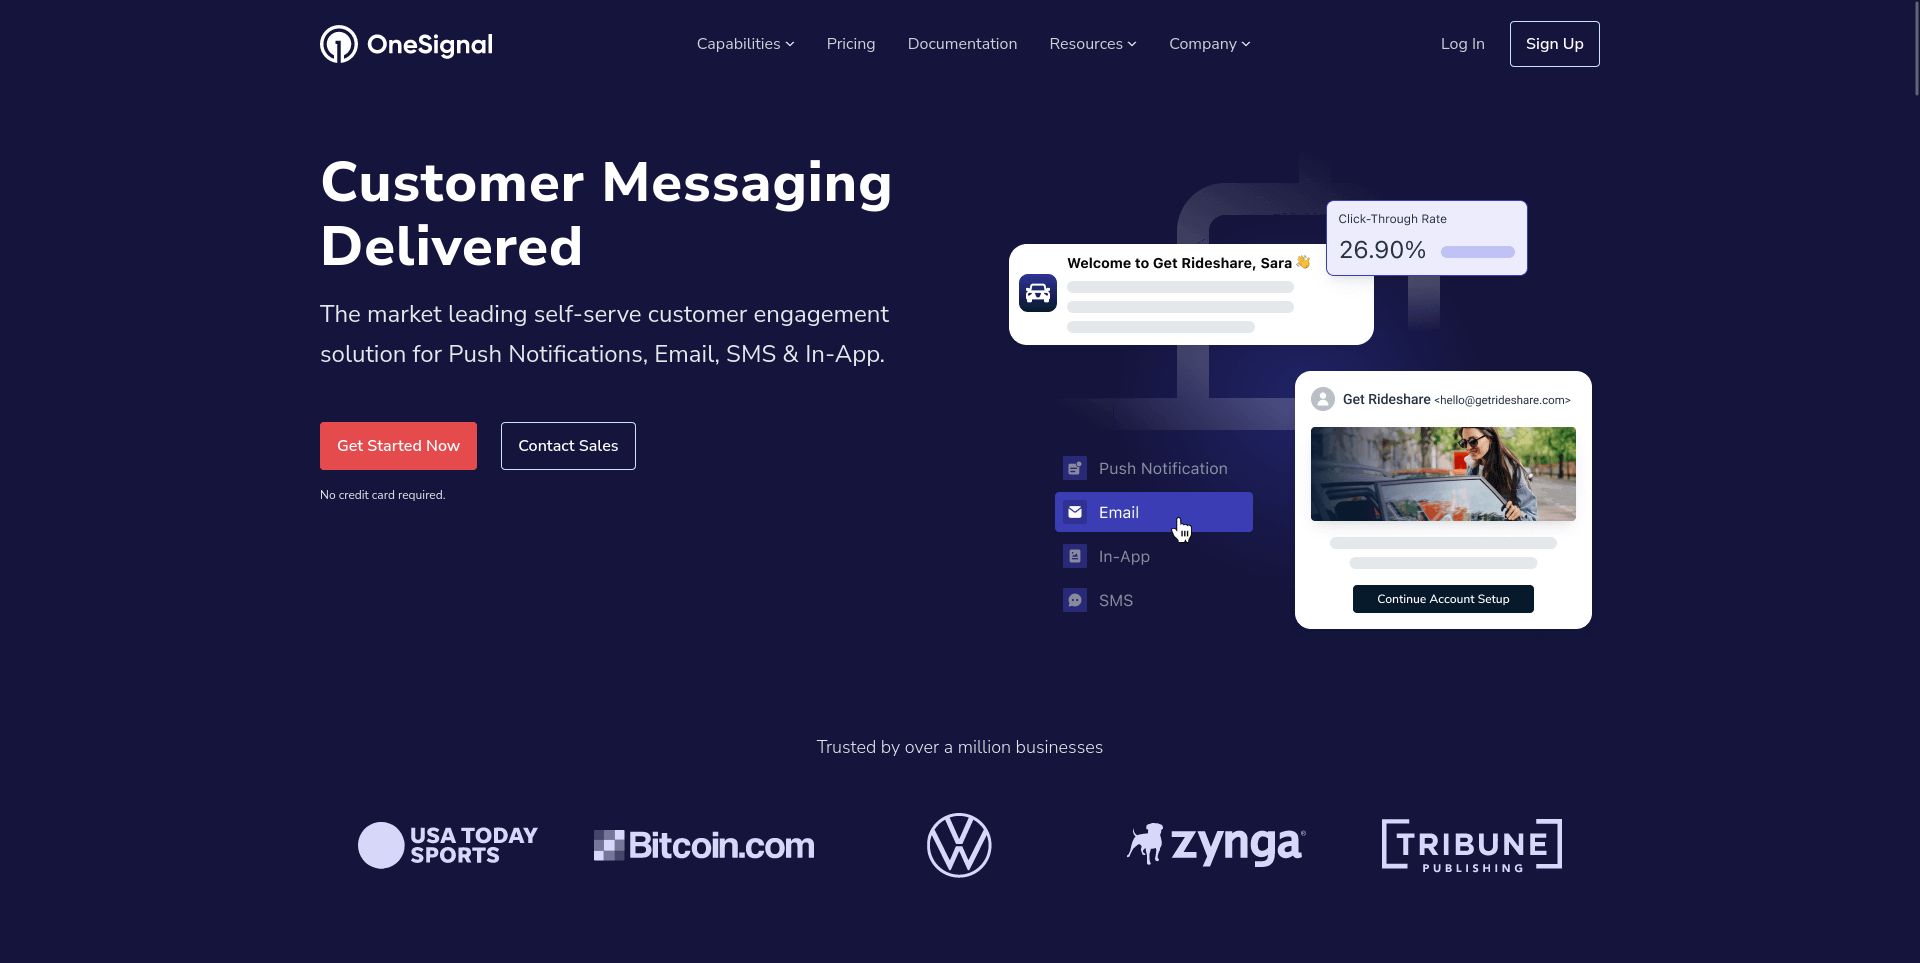
\includegraphics[width=0.8\textwidth]{onesignal.png}
    \caption{OneSignal Homepage}
\end{figure}

\subsubsection{Pusher}
Pusher is a cloud-based notification service that provides real-time messaging for mobile and web applications.
It supports push notifications, in-app notifications, and allows integration with other services and platforms. \\

\begin{figure}[hbt!]
    \centering
    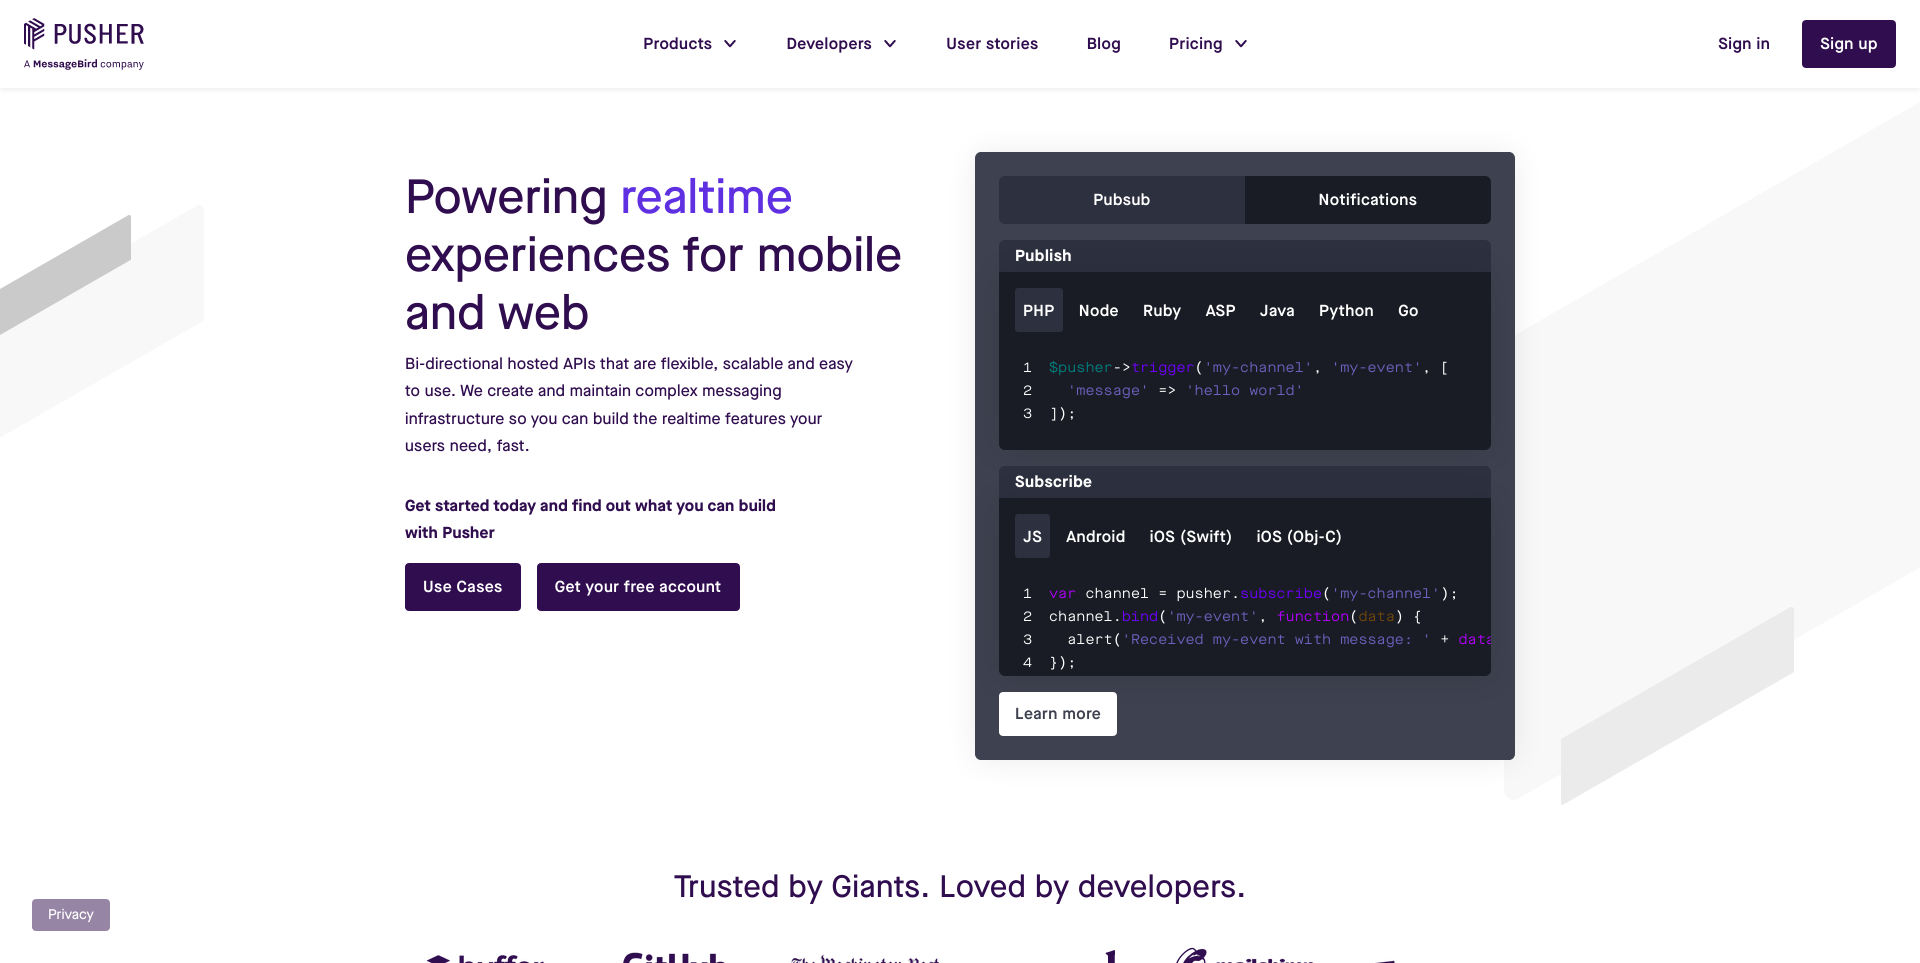
\includegraphics[width=0.8\textwidth]{pusher.png}
    \caption{Pusher Homepage}
\end{figure}

\subsubsection{Amazon SNS}
Amazon SNS (Simple Notification Service) is a fully managed messaging service provided by Amazon Web 
Services (AWS) that enables you to send messages or notifications to a variety of distributed endpoints 
or clients. \\

\begin{figure}[hbt!]
    \centering
    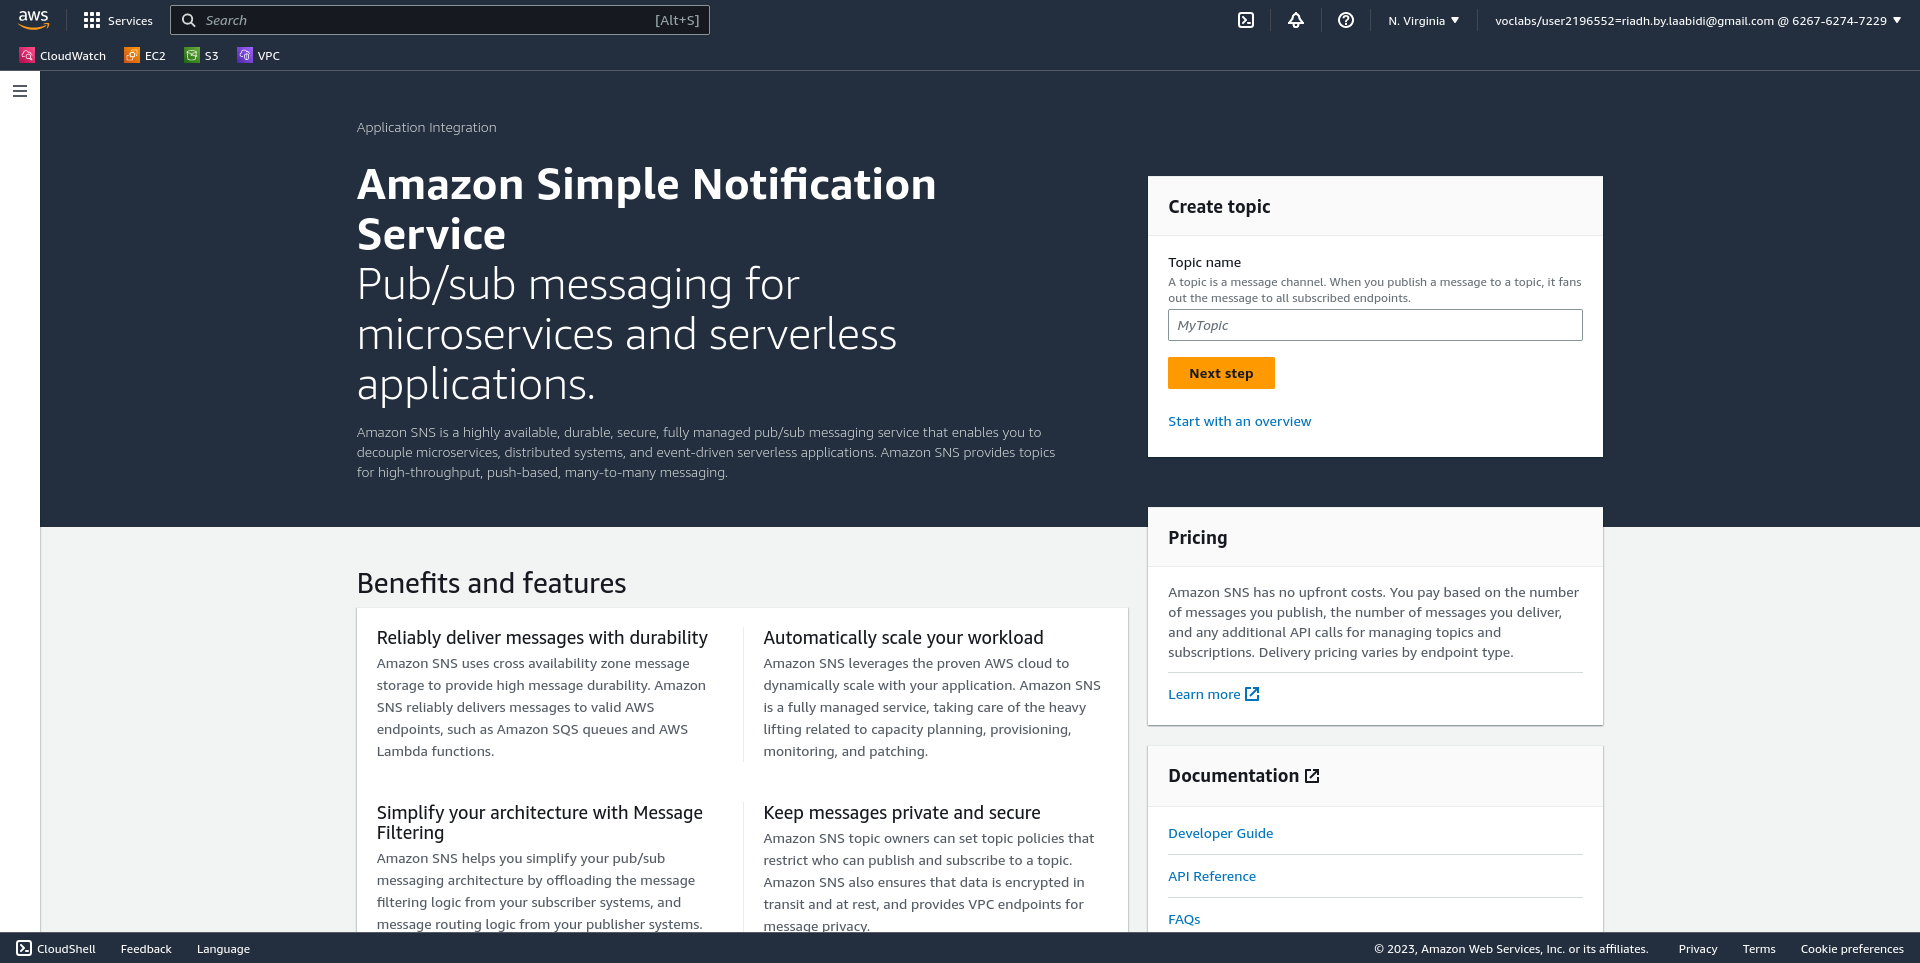
\includegraphics[width=0.8\textwidth]{amazonsns.png}
    \caption{Amazon SNS Service Homepage}
\end{figure}

\subsection{Comparison}
We will conduct a comprehensive analysis of the selected existing solutions.
By thoroughly examining their functionalities, strengths, and weaknesses, we aim to gain valuable insights 
into areas where improvements can be made to enhance user experience, streamline processes, and deliver 
a superior solution tailored to our specific requirements.

Our evaluation will be based on 6 criterias (Cx) that have been carefully selected as being the most 
relevant and aligned with the Convergence project requirements:

\begin{itemize}
    \item \textbf{C1: Multi-channel delivery:} The ability to configure multiple channels (Email, SMS, 
    Push, Chat) for notification delivery.
    \item \textbf{C2: Deliverability:} Ensuring that notifications and alerts are successfully delivered 
    to users' devices.
    \item \textbf{C3: User Segmentation:} The ability to select and target specific groups of users based on 
    criterias defined by the business requirements.
    \item \textbf{C4: Customization:}  The ability to customize notifications content for targeted users accordingly.
    \item \textbf{C5: Analytics:} The ability to track different metrics during the delivery process 
    in order to inform businesses about the effectiveness of notification campaings and improve user engagement.
    \item \textbf{C6: Cost:} Charge per sent notifications for a larger user base and high notification volume.
    \item \textbf{C7: Ease of use:} The ability to easily setup and configure the different steps of the notification
    delivery process for non technical users.
\end{itemize} 

\begin{table}[hbt!]
    \centering
    \begin{tabularx}{\textwidth}{ |
        >{\raggedright\arraybackslash} X | 
        >{\raggedright\arraybackslash} X |
        >{\raggedright\arraybackslash} X | 
        >{\raggedright\arraybackslash} X | 
        }
        \hline
         & \textbf{OneSignal} & \textbf{Pusher} & \textbf{Amazon SNS}  \\
        \hline
        \textbf{C1} \linebreak Multi-channel delivery & Provides most of channels (Push, Email, SMS), except for the Chat channel & Provides Push 
        (Android, iOS, Web) notifications only
         & Does not provide native support for multi-channel notifications  \\
        \hline
        \textbf{C2} \linebreak Deliverability & Low \acrshort{ctr} and drops over time due to inactive receivers leading to misinformation for senders about the deliverability of their notifications.  &  &  \\
        \hline
        \textbf{C3} \linebreak User Segmentation & & & Does not support targeting specific segments of users based on their behavior or preferences. \\
        \hline
        \textbf{C4} \linebreak Customization & \textbf{Limited}: Users can’t fully customize the layout of the notification.  & \textbf{Limited}: Only a subject and a body, no dynamic content. & \textbf{Limited}: Only text message, subject and body, no dynamic content.
        \\
        \hline
        \textbf{C5} \linebreak Analytics  & & & No detailed insights on sent notifications \\
        \hline 
        \textbf{C6} \linebreak Cost & \textbf{249\$/month} (for 50,000 subscribers from push notifications only) & \textbf{99\$/month} for 50,000 subscribers & Charge per usage (Pay as you go) \\
        \hline
        \textbf{C7} \linebreak Ease of use & & Mostly Programmatic, does not provide a fully featured web interface. & Complex and time-consuming particularly for non technical users. \\
        \hline
     \end{tabularx}
    \caption{Comparison table}
\end{table}

\section{Work methodology}
With today’s customers and businesses requiring rapid responses and changes, teams at Satoripop are embracing 
the Agile methodology, a project management approach that involves breaking the project into phases 
and emphasizes continuous collaboration and improvement, following a cycle of planning, executing, 
and evaluating. 

One of the frameworks that helps practice building the mentioned agile priciples into work and that we will 
be focusing on is Scrum. we will provide an overview of this framework, highlighting its approach and 
key principles

\subsection{The scrum framework}
Scrum is a lightweight framework that helps people, teams and organizations generate value through adaptive 
solutions for complex problems. It employs an iterative, incremental approach to optimize predictability 
and to control risk, while engages groups of people who collectively have all the skills and expertise 
to do the work and share or acquire such skills as needed.

\subsection{Members of a scrum team }
The fundamental unit of Scrum is a small team of people. The Scrum Team consists of
one Scrum Master, one Product Owner, and Developers. Within a Scrum Team, there are no sub-teams
or hierarchies. It is a cohesive unit of professionals focused on one objective at a time, 
the Product Goal. \cite{scrumguides}

\begin{itemize}
    \item \textbf{Developers:} People in the Scrum Team that are committed to creating any aspect 
    of a usable Increment each Sprint.
    \item \textbf{Product Owner:} One person that may represent the needs of many stakeholders
    in the Product Backlog. The Product Owner is accountable for effective Product Backlog management 
    and maximizing the value of the product resulting from the work of the Scrum Team.
    \item \textbf{Scrum Master:} Deeply understands the work being done by the team and 
    can help the team optimize their transparency and delivery flow. As the facilitator-in-chief, 
    he/she schedules the needed resources (both human and logistical) for sprint planning, stand-up, 
    sprint review, and the sprint retrospective.
\end{itemize}
\raggedbottom

\subsection{Scrum events}
The Sprint is a container for all other events. Each event in Scrum is a formal opportunity to inspect 
and adapt Scrum artifacts. These events are specifically designed to enable the transparency required.

\begin{itemize}
    \item \textbf{The Sprint:} Sprints are the heartbeat of Scrum, where ideas are turned into value. 
    They are fixed length events of one month or less to create consistency. A new Sprint starts 
    immediately after the conclusion of the previous Sprint.
    \item \textbf{Sprint Planning} The work to be performed during the current sprint is planned during 
    this meeting by the entire development team. Specific user stories are then added to the sprint from 
    the product backlog. These stories always align with the goal and are also agreed upon by the scrum 
    team to be feasible to implement.
    \item \textbf{Daily Scrum:} A 15-minute event for the Developers of the Scrum Team 
    held every working day of the Sprint to inspect progress toward the Sprint Goal and adapt the Sprint
    Backlog as necessary.
    \item \textbf{Sprint Review:} The purpose of the Sprint Review is to inspect the outcome of the 
    Sprint and determine future adaptations. The Scrum Team presents the results of their work to key 
    stakeholders and progress toward the Product Goal is discussed.
    \item \textbf{Sprint Retrospective:} The purpose of the Sprint Retrospective is to plan ways to 
    increase quality and effectiveness. The Scrum Team identifies the most helpful changes to improve 
    its effectiveness and these changes are addressed as soon as possible.
\end{itemize}


\subsection{Scrum artifacts}
Scrum’s artifacts represent work or value. They are designed to maximize transparency of key information. 
Thus, everyone inspecting them has the same basis for adaptation.

\begin{itemize}
    \item \textbf{Product Backlog:} The primary list of work that needs to get done. It's a dynamic list 
    of features, enhancements, and fixes that acts as the input for the sprint backlog. 
    This list is constantly revisited, re-prioritized and maintained by the Product Owner in case items 
    may no longer be relevant or problems may get solved in other ways.
    \item \textbf{Sprint Backlog:} The list of items, user stories, or bug fixes, selected by the 
    development team for implementation in the current sprint cycle. A sprint backlog may be flexible 
    and can evolve during a sprint without compromising the fundamental sprint goal.
    \item \textbf{Increment:} A concrete stepping stone toward the Product Goal. 
    Each Increment is additive to all prior Increments and thoroughly verified, ensuring that all 
    Increments work together. In order to provide value, the Increment must be usable.
\end{itemize}
\raggedbottom

\phantomsection
\section*{Summary}
\addcontentsline{toc}{section}{Summary}
To summarize our findings in this chapter, we introduced the host organization, then outlined the problem 
assessment and identified its related challenges. Next we analyzed competitors to get a grasp of the major
pain points that we are going to tackle, and finally we presented the adopted agile approach in our team
to foster flexibility and collaboration. 

The next chapter will introduce the Sprint 0, where we kickstart the project, establish goals, and set 
the roadmap for upcoming sprints.



